% Options for packages loaded elsewhere
\PassOptionsToPackage{unicode}{hyperref}
\PassOptionsToPackage{hyphens}{url}
\PassOptionsToPackage{dvipsnames,svgnames,x11names}{xcolor}
%
\documentclass[
  letterpaper,
  DIV=11,
  numbers=noendperiod]{scrartcl}

\usepackage{amsmath,amssymb}
\usepackage{iftex}
\ifPDFTeX
  \usepackage[T1]{fontenc}
  \usepackage[utf8]{inputenc}
  \usepackage{textcomp} % provide euro and other symbols
\else % if luatex or xetex
  \usepackage{unicode-math}
  \defaultfontfeatures{Scale=MatchLowercase}
  \defaultfontfeatures[\rmfamily]{Ligatures=TeX,Scale=1}
\fi
\usepackage{lmodern}
\ifPDFTeX\else  
    % xetex/luatex font selection
\fi
% Use upquote if available, for straight quotes in verbatim environments
\IfFileExists{upquote.sty}{\usepackage{upquote}}{}
\IfFileExists{microtype.sty}{% use microtype if available
  \usepackage[]{microtype}
  \UseMicrotypeSet[protrusion]{basicmath} % disable protrusion for tt fonts
}{}
\makeatletter
\@ifundefined{KOMAClassName}{% if non-KOMA class
  \IfFileExists{parskip.sty}{%
    \usepackage{parskip}
  }{% else
    \setlength{\parindent}{0pt}
    \setlength{\parskip}{6pt plus 2pt minus 1pt}}
}{% if KOMA class
  \KOMAoptions{parskip=half}}
\makeatother
\usepackage{xcolor}
\setlength{\emergencystretch}{3em} % prevent overfull lines
\setcounter{secnumdepth}{5}
% Make \paragraph and \subparagraph free-standing
\ifx\paragraph\undefined\else
  \let\oldparagraph\paragraph
  \renewcommand{\paragraph}[1]{\oldparagraph{#1}\mbox{}}
\fi
\ifx\subparagraph\undefined\else
  \let\oldsubparagraph\subparagraph
  \renewcommand{\subparagraph}[1]{\oldsubparagraph{#1}\mbox{}}
\fi

\usepackage{color}
\usepackage{fancyvrb}
\newcommand{\VerbBar}{|}
\newcommand{\VERB}{\Verb[commandchars=\\\{\}]}
\DefineVerbatimEnvironment{Highlighting}{Verbatim}{commandchars=\\\{\}}
% Add ',fontsize=\small' for more characters per line
\usepackage{framed}
\definecolor{shadecolor}{RGB}{241,243,245}
\newenvironment{Shaded}{\begin{snugshade}}{\end{snugshade}}
\newcommand{\AlertTok}[1]{\textcolor[rgb]{0.68,0.00,0.00}{#1}}
\newcommand{\AnnotationTok}[1]{\textcolor[rgb]{0.37,0.37,0.37}{#1}}
\newcommand{\AttributeTok}[1]{\textcolor[rgb]{0.40,0.45,0.13}{#1}}
\newcommand{\BaseNTok}[1]{\textcolor[rgb]{0.68,0.00,0.00}{#1}}
\newcommand{\BuiltInTok}[1]{\textcolor[rgb]{0.00,0.23,0.31}{#1}}
\newcommand{\CharTok}[1]{\textcolor[rgb]{0.13,0.47,0.30}{#1}}
\newcommand{\CommentTok}[1]{\textcolor[rgb]{0.37,0.37,0.37}{#1}}
\newcommand{\CommentVarTok}[1]{\textcolor[rgb]{0.37,0.37,0.37}{\textit{#1}}}
\newcommand{\ConstantTok}[1]{\textcolor[rgb]{0.56,0.35,0.01}{#1}}
\newcommand{\ControlFlowTok}[1]{\textcolor[rgb]{0.00,0.23,0.31}{#1}}
\newcommand{\DataTypeTok}[1]{\textcolor[rgb]{0.68,0.00,0.00}{#1}}
\newcommand{\DecValTok}[1]{\textcolor[rgb]{0.68,0.00,0.00}{#1}}
\newcommand{\DocumentationTok}[1]{\textcolor[rgb]{0.37,0.37,0.37}{\textit{#1}}}
\newcommand{\ErrorTok}[1]{\textcolor[rgb]{0.68,0.00,0.00}{#1}}
\newcommand{\ExtensionTok}[1]{\textcolor[rgb]{0.00,0.23,0.31}{#1}}
\newcommand{\FloatTok}[1]{\textcolor[rgb]{0.68,0.00,0.00}{#1}}
\newcommand{\FunctionTok}[1]{\textcolor[rgb]{0.28,0.35,0.67}{#1}}
\newcommand{\ImportTok}[1]{\textcolor[rgb]{0.00,0.46,0.62}{#1}}
\newcommand{\InformationTok}[1]{\textcolor[rgb]{0.37,0.37,0.37}{#1}}
\newcommand{\KeywordTok}[1]{\textcolor[rgb]{0.00,0.23,0.31}{#1}}
\newcommand{\NormalTok}[1]{\textcolor[rgb]{0.00,0.23,0.31}{#1}}
\newcommand{\OperatorTok}[1]{\textcolor[rgb]{0.37,0.37,0.37}{#1}}
\newcommand{\OtherTok}[1]{\textcolor[rgb]{0.00,0.23,0.31}{#1}}
\newcommand{\PreprocessorTok}[1]{\textcolor[rgb]{0.68,0.00,0.00}{#1}}
\newcommand{\RegionMarkerTok}[1]{\textcolor[rgb]{0.00,0.23,0.31}{#1}}
\newcommand{\SpecialCharTok}[1]{\textcolor[rgb]{0.37,0.37,0.37}{#1}}
\newcommand{\SpecialStringTok}[1]{\textcolor[rgb]{0.13,0.47,0.30}{#1}}
\newcommand{\StringTok}[1]{\textcolor[rgb]{0.13,0.47,0.30}{#1}}
\newcommand{\VariableTok}[1]{\textcolor[rgb]{0.07,0.07,0.07}{#1}}
\newcommand{\VerbatimStringTok}[1]{\textcolor[rgb]{0.13,0.47,0.30}{#1}}
\newcommand{\WarningTok}[1]{\textcolor[rgb]{0.37,0.37,0.37}{\textit{#1}}}

\providecommand{\tightlist}{%
  \setlength{\itemsep}{0pt}\setlength{\parskip}{0pt}}\usepackage{longtable,booktabs,array}
\usepackage{calc} % for calculating minipage widths
% Correct order of tables after \paragraph or \subparagraph
\usepackage{etoolbox}
\makeatletter
\patchcmd\longtable{\par}{\if@noskipsec\mbox{}\fi\par}{}{}
\makeatother
% Allow footnotes in longtable head/foot
\IfFileExists{footnotehyper.sty}{\usepackage{footnotehyper}}{\usepackage{footnote}}
\makesavenoteenv{longtable}
\usepackage{graphicx}
\makeatletter
\def\maxwidth{\ifdim\Gin@nat@width>\linewidth\linewidth\else\Gin@nat@width\fi}
\def\maxheight{\ifdim\Gin@nat@height>\textheight\textheight\else\Gin@nat@height\fi}
\makeatother
% Scale images if necessary, so that they will not overflow the page
% margins by default, and it is still possible to overwrite the defaults
% using explicit options in \includegraphics[width, height, ...]{}
\setkeys{Gin}{width=\maxwidth,height=\maxheight,keepaspectratio}
% Set default figure placement to htbp
\makeatletter
\def\fps@figure{htbp}
\makeatother

% load packages
\usepackage{geometry}
\usepackage{xcolor}
\usepackage{eso-pic}
\usepackage{fancyhdr}
\usepackage{sectsty}
\usepackage{fontspec}
\usepackage{titlesec}

%% Set page size with a wider right margin
\geometry{a4paper, total={170mm,257mm}, left=20mm, top=20mm, bottom=20mm, right=50mm}

%% Let's define some colours
\definecolor{uniblue}{HTML}{003865}
\definecolor{burgundy}{HTML}{7D2239}
\definecolor{cobalt}{HTML}{005C8A}
\definecolor{lavender}{HTML}{5B4D94}
\definecolor{leaf}{HTML}{006630}
\definecolor{moss}{HTML}{385A4F}
\definecolor{pillarbox}{HTML}{B30C00}
\definecolor{rust}{HTML}{9A3A06}
\definecolor{sandstone}{HTML}{52473B}
\definecolor{skyblue}{HTML}{005398}
\definecolor{slate}{HTML}{4F5961}
\definecolor{thistle}{HTML}{951272}

%\definecolor{light}{HTML}{E6E6FA} % original from template - redefined below as uni blue at 10 percent:
\colorlet{light}{uniblue!10}
%\definecolor{highlight}{HTML}{800080} % original from template - redefined below as uni's skyblue:
\colorlet{highlight}{skyblue}
%\definecolor{dark}{HTML}{330033} % original from template - redefined below as uni blue at 100 percent:
\colorlet{dark}{uniblue}

%% Let's add the border on the right hand side 
\AddToShipoutPicture{% 
    \AtPageLowerLeft{% 
        \put(\LenToUnit{\dimexpr\paperwidth-3cm},0){% 
            \color{light}\rule{3cm}{\LenToUnit\paperheight}%
          }%
     }%
     % logo
    \AtPageLowerLeft{% start the bar at the bottom right of the page
        \put(\LenToUnit{\dimexpr\paperwidth-2.25cm},27.2cm){% move it to the top right
            \color{light}
\includegraphics[width=2.25cm]{_extensions/nrennie/PrettyPDF/uni_logo_boxed.jpg}
          }%
     }%
}

%% Style the page number
\fancypagestyle{mystyle}{
  \fancyhf{}
  \renewcommand\headrulewidth{0pt}
  \fancyfoot[R]{\thepage}
  \fancyfootoffset{3.5cm}
}
\setlength{\footskip}{20pt}

%% style the chapter/section fonts
\chapterfont{\color{uniblue}\fontsize{20}{16.8}\selectfont}
\sectionfont{\color{uniblue}\fontsize{20}{16.8}\selectfont}
\subsectionfont{\color{skyblue}\fontsize{14}{16.8}\selectfont}
\titleformat{\subsection}
  {\color{uniblue!90}\sffamily\Large\bfseries}{\thesubsection}{1em}{}[{\titlerule[0.8pt]}]
\subsubsectionfont{\color{cobalt}}

\renewcommand\thesection{\color{slate}\arabic{section}}
  
% left align title
\makeatletter
\renewcommand{\maketitle}{\bgroup\setlength{\parindent}{0pt}
\begin{flushleft}
  {\color{uniblue}\sffamily\huge\textbf{\@title}} \vspace{0.3cm} \newline
  {\Large {\@subtitle}} \newline
  \@author
\end{flushleft}\egroup
}
\makeatother

%% Use some custom fonts
\setsansfont{Ubuntu}[
    Path=_extensions/nrennie/PrettyPDF/Ubuntu/,
    Scale=0.9,
    Extension = .ttf,
    UprightFont=*-Regular,
    BoldFont=*-Bold,
    ItalicFont=*-Italic,
    ]

\setmainfont{Ubuntu}[
    Path=_extensions/nrennie/PrettyPDF/Ubuntu/,
    Scale=0.9,
    Extension = .ttf,
    UprightFont=*-Regular,
    BoldFont=*-Bold,
    ItalicFont=*-Italic,
    ]
\KOMAoption{captions}{tableheading}
\makeatletter
\@ifpackageloaded{tcolorbox}{}{\usepackage[skins,breakable]{tcolorbox}}
\@ifpackageloaded{fontawesome5}{}{\usepackage{fontawesome5}}
\definecolor{quarto-callout-color}{HTML}{909090}
\definecolor{quarto-callout-note-color}{HTML}{0758E5}
\definecolor{quarto-callout-important-color}{HTML}{CC1914}
\definecolor{quarto-callout-warning-color}{HTML}{EB9113}
\definecolor{quarto-callout-tip-color}{HTML}{00A047}
\definecolor{quarto-callout-caution-color}{HTML}{FC5300}
\definecolor{quarto-callout-color-frame}{HTML}{acacac}
\definecolor{quarto-callout-note-color-frame}{HTML}{4582ec}
\definecolor{quarto-callout-important-color-frame}{HTML}{d9534f}
\definecolor{quarto-callout-warning-color-frame}{HTML}{f0ad4e}
\definecolor{quarto-callout-tip-color-frame}{HTML}{02b875}
\definecolor{quarto-callout-caution-color-frame}{HTML}{fd7e14}
\makeatother
\makeatletter
\@ifpackageloaded{caption}{}{\usepackage{caption}}
\AtBeginDocument{%
\ifdefined\contentsname
  \renewcommand*\contentsname{Table of contents}
\else
  \newcommand\contentsname{Table of contents}
\fi
\ifdefined\listfigurename
  \renewcommand*\listfigurename{List of Figures}
\else
  \newcommand\listfigurename{List of Figures}
\fi
\ifdefined\listtablename
  \renewcommand*\listtablename{List of Tables}
\else
  \newcommand\listtablename{List of Tables}
\fi
\ifdefined\figurename
  \renewcommand*\figurename{Figure}
\else
  \newcommand\figurename{Figure}
\fi
\ifdefined\tablename
  \renewcommand*\tablename{Table}
\else
  \newcommand\tablename{Table}
\fi
}
\@ifpackageloaded{float}{}{\usepackage{float}}
\floatstyle{ruled}
\@ifundefined{c@chapter}{\newfloat{codelisting}{h}{lop}}{\newfloat{codelisting}{h}{lop}[chapter]}
\floatname{codelisting}{Listing}
\newcommand*\listoflistings{\listof{codelisting}{List of Listings}}
\makeatother
\makeatletter
\makeatother
\makeatletter
\@ifpackageloaded{caption}{}{\usepackage{caption}}
\@ifpackageloaded{subcaption}{}{\usepackage{subcaption}}
\makeatother
\makeatletter
\@ifpackageloaded{tcolorbox}{}{\usepackage[skins,breakable]{tcolorbox}}
\makeatother
\makeatletter
\@ifundefined{shadecolor}{\definecolor{shadecolor}{rgb}{.97, .97, .97}}{}
\makeatother
\makeatletter
\@ifundefined{codebgcolor}{\definecolor{codebgcolor}{named}{light}}{}
\makeatother
\makeatletter
\ifdefined\Shaded\renewenvironment{Shaded}{\begin{tcolorbox}[enhanced, breakable, colback={codebgcolor}, frame hidden, boxrule=0pt, sharp corners]}{\end{tcolorbox}}\fi
\makeatother
\ifLuaTeX
  \usepackage{selnolig}  % disable illegal ligatures
\fi
\usepackage{bookmark}

\IfFileExists{xurl.sty}{\usepackage{xurl}}{} % add URL line breaks if available
\urlstyle{same} % disable monospaced font for URLs
\hypersetup{
  pdftitle={Week 4 Tasks},
  colorlinks=true,
  linkcolor={highlight},
  filecolor={Maroon},
  citecolor={Blue},
  urlcolor={highlight},
  pdfcreator={LaTeX via pandoc}}

\title{Week 4 Tasks}
\author{}
\date{}

\begin{document}
\maketitle

\pagestyle{mystyle}

\section{Tasks}\label{tasks}

You are encouraged to complete the following tasks by using Quarto to
produce a single document which summarises all your work, i.e.~the
original questions, your R code, your comments and reflections, etc.

\subsection{Part 1}\label{part-1}

Data was collected on the characteristics of homes in the American city
of Los Angeles (LA) in 2010 and can be downloaded below:

The data contain the following variables:

\begin{itemize}
\item
  \texttt{city} - the district of LA where the house was located
\item
  \texttt{type} - either \texttt{SFR} (Single Family Residences) or
  \texttt{Condo/Twh} (Condominium/Town House)
\item
  \texttt{bed} - the number of bedrooms
\item
  \texttt{bath} - the number of bathrooms
\item
  \texttt{garage} - the number of car spaces in the garage
\item
  \texttt{sqft} - the floor area of the house (in square feet)
\item
  \texttt{pool} - \texttt{Y} if the house has a pool
\item
  \texttt{spa} - \texttt{TRUE} if the house has a spa
\item
  \texttt{price} - the most recent sales price (\$US)
\end{itemize}

We are interested in exploring the relationships between \texttt{price}
and the other variables.

Read the data into an object called \texttt{LAhomes} and complete the
following tasks

\begin{Shaded}
\begin{Highlighting}[]
\NormalTok{LAhomes }\OtherTok{\textless{}{-}} \FunctionTok{read.csv}\NormalTok{(}\StringTok{"LAhomes.csv"}\NormalTok{,}\AttributeTok{stringsAsFactors =}\NormalTok{ T)}
\end{Highlighting}
\end{Shaded}

\begin{tcolorbox}[enhanced jigsaw, toprule=.15mm, breakable, bottomtitle=1mm, coltitle=black, colback=white, arc=.35mm, left=2mm, leftrule=.75mm, opacitybacktitle=0.6, colframe=quarto-callout-warning-color-frame, colbacktitle=quarto-callout-warning-color!10!white, toptitle=1mm, titlerule=0mm, opacityback=0, title={Task 1}, rightrule=.15mm, bottomrule=.15mm]

By looking at the univariate and bivariate distributions on the
\texttt{price} and \texttt{sqft} variables below, what would be a
sensible way to proceed if we wanted to model this data? What care must
be taken if you were to proceed this way?

Click here to see the solution

\begin{Shaded}
\begin{Highlighting}[]
\NormalTok{hist1 }\OtherTok{\textless{}{-}} \FunctionTok{ggplot}\NormalTok{(LAhomes, }\FunctionTok{aes}\NormalTok{(}\AttributeTok{x =}\NormalTok{ price)) }\SpecialCharTok{+}
          \FunctionTok{geom\_histogram}\NormalTok{()}
\NormalTok{hist2 }\OtherTok{\textless{}{-}} \FunctionTok{ggplot}\NormalTok{(LAhomes, }\FunctionTok{aes}\NormalTok{(}\AttributeTok{x =}\NormalTok{ sqft)) }\SpecialCharTok{+}
          \FunctionTok{geom\_histogram}\NormalTok{()}

\CommentTok{\# Explore log transformation}
\NormalTok{hist1log }\OtherTok{\textless{}{-}} \FunctionTok{ggplot}\NormalTok{(LAhomes, }\FunctionTok{aes}\NormalTok{(}\AttributeTok{x =} \FunctionTok{log}\NormalTok{(price))) }\SpecialCharTok{+}
             \FunctionTok{geom\_histogram}\NormalTok{()}
\NormalTok{hist2log }\OtherTok{\textless{}{-}} \FunctionTok{ggplot}\NormalTok{(LAhomes, }\FunctionTok{aes}\NormalTok{(}\AttributeTok{x =} \FunctionTok{log}\NormalTok{(sqft))) }\SpecialCharTok{+}
             \FunctionTok{geom\_histogram}\NormalTok{()}

\NormalTok{plot1 }\OtherTok{\textless{}{-}} \FunctionTok{ggplot}\NormalTok{(LAhomes, }\FunctionTok{aes}\NormalTok{(}\AttributeTok{x =}\NormalTok{ sqft, }\AttributeTok{y =}\NormalTok{ price)) }\SpecialCharTok{+}
          \FunctionTok{geom\_point}\NormalTok{()}
\NormalTok{plot2 }\OtherTok{\textless{}{-}} \FunctionTok{ggplot}\NormalTok{(LAhomes, }\FunctionTok{aes}\NormalTok{(}\AttributeTok{x =} \FunctionTok{log}\NormalTok{(sqft), }\AttributeTok{y =} \FunctionTok{log}\NormalTok{(price))) }\SpecialCharTok{+}
          \FunctionTok{geom\_point}\NormalTok{()}

\FunctionTok{grid.arrange}\NormalTok{(hist1, hist2, hist1log, hist2log, plot1, plot2,}
             \AttributeTok{ncol =} \DecValTok{2}\NormalTok{, }\AttributeTok{nrow =} \DecValTok{3}\NormalTok{)}
\end{Highlighting}
\end{Shaded}

\begin{center}
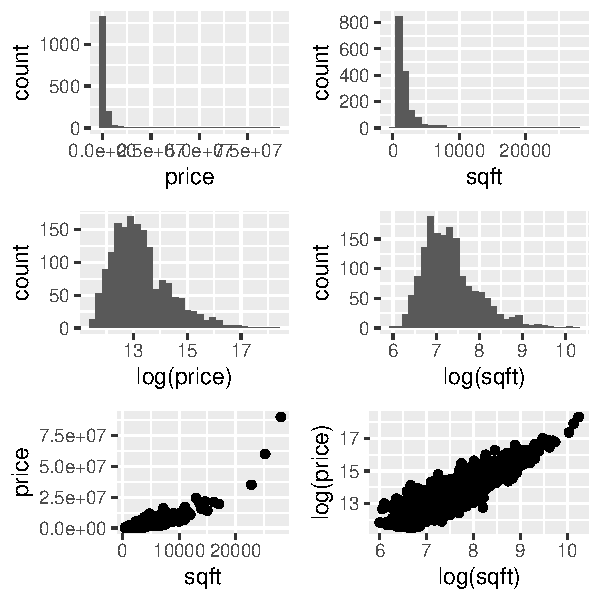
\includegraphics{about_files/figure-pdf/unnamed-chunk-3-1.pdf}
\end{center}

\end{tcolorbox}

\begin{tcolorbox}[enhanced jigsaw, toprule=.15mm, breakable, bottomtitle=1mm, coltitle=black, colback=white, arc=.35mm, left=2mm, leftrule=.75mm, opacitybacktitle=0.6, colframe=quarto-callout-warning-color-frame, colbacktitle=quarto-callout-warning-color!10!white, toptitle=1mm, titlerule=0mm, opacityback=0, title={Task 2}, rightrule=.15mm, bottomrule=.15mm]

Fit the simple linear model with \texttt{log(price)} as the response and
\texttt{log(sqft)} as the predictor. Display the fitted model on a
scatterplot of the data and construct a confidence interval for the
slope parameter in the model and interpret its point and interval
estimates.

Click here to see the solution

\begin{Shaded}
\begin{Highlighting}[]
\NormalTok{slr\_LAprices }\OtherTok{\textless{}{-}} \FunctionTok{lm}\NormalTok{(}\FunctionTok{log}\NormalTok{(price) }\SpecialCharTok{\textasciitilde{}} \FunctionTok{log}\NormalTok{(sqft), }\AttributeTok{data =}\NormalTok{ LAhomes)}

\FunctionTok{ggplot}\NormalTok{(LAhomes, }\FunctionTok{aes}\NormalTok{(}\AttributeTok{x =}  \FunctionTok{log}\NormalTok{(sqft), }\AttributeTok{y =} \FunctionTok{log}\NormalTok{(price))) }\SpecialCharTok{+}
  \FunctionTok{geom\_point}\NormalTok{(}\AttributeTok{alpha=}\FloatTok{0.25}\NormalTok{) }\SpecialCharTok{+}
  \FunctionTok{labs}\NormalTok{(}\AttributeTok{x =} \StringTok{"log(aquare feet)"}\NormalTok{, }\AttributeTok{y =} \StringTok{"log(price)"}\NormalTok{) }\SpecialCharTok{+}
  \FunctionTok{geom\_smooth}\NormalTok{(}\AttributeTok{method =} \StringTok{"lm"}\NormalTok{, }\AttributeTok{level =}\FloatTok{0.95}\NormalTok{)}
\end{Highlighting}
\end{Shaded}

\begin{center}
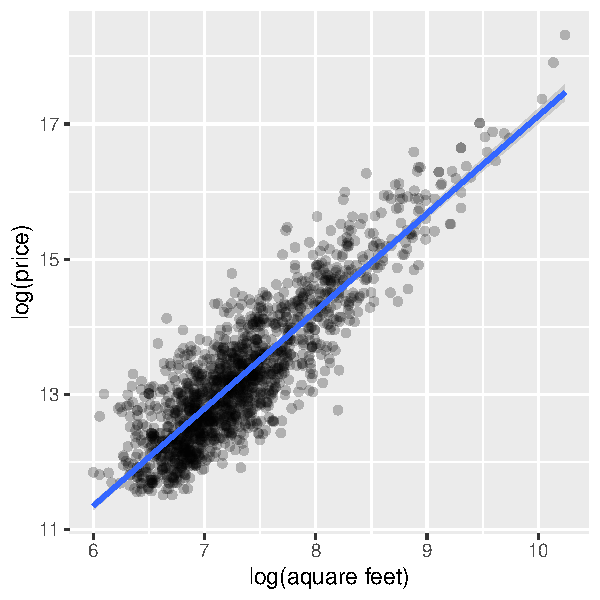
\includegraphics{about_files/figure-pdf/unnamed-chunk-4-1.pdf}
\end{center}

\begin{Shaded}
\begin{Highlighting}[]
\FunctionTok{tab\_model}\NormalTok{(slr\_LAprices)}
\end{Highlighting}
\end{Shaded}

\begin{longtable}[]{@{}cccc@{}}
\toprule\noalign{}
\endhead
\bottomrule\noalign{}
\endlastfoot
~ & \multicolumn{3}{c@{}}{%
log(price)} \\
Predictors & Estimates & CI & p \\
(Intercept) & 2.70 & 2.42~--~2.98 & \textbf{\textless0.001} \\
sqft {[}log{]} & 1.44 & 1.40~--~1.48 & \textbf{\textless0.001} \\
Observations & \multicolumn{3}{l@{}}{%
1594} \\
R\textsuperscript{2} / R\textsuperscript{2} adjusted &
\multicolumn{3}{l@{}}{%
0.774 / 0.774} \\
\end{longtable}

\end{tcolorbox}

\begin{tcolorbox}[enhanced jigsaw, toprule=.15mm, breakable, bottomtitle=1mm, coltitle=black, colback=white, arc=.35mm, left=2mm, leftrule=.75mm, opacitybacktitle=0.6, colframe=quarto-callout-warning-color-frame, colbacktitle=quarto-callout-warning-color!10!white, toptitle=1mm, titlerule=0mm, opacityback=0, title={Task 3}, rightrule=.15mm, bottomrule=.15mm]

Re-do your analysis but now using \texttt{log(bath)} as the explanatory
variable. Calculate the point and interval estimates of the
coefficients.

Click here to see the solution

\begin{Shaded}
\begin{Highlighting}[]
\NormalTok{slr\_LAprices2 }\OtherTok{\textless{}{-}} \FunctionTok{lm}\NormalTok{(}\FunctionTok{log}\NormalTok{(price) }\SpecialCharTok{\textasciitilde{}} \FunctionTok{log}\NormalTok{(bath), }\AttributeTok{data =}\NormalTok{ LAhomes)}

\FunctionTok{ggplot}\NormalTok{(LAhomes, }\FunctionTok{aes}\NormalTok{(}\AttributeTok{x =}  \FunctionTok{log}\NormalTok{(bath), }\AttributeTok{y =} \FunctionTok{log}\NormalTok{(price))) }\SpecialCharTok{+}
  \FunctionTok{geom\_point}\NormalTok{(}\AttributeTok{alpha=}\FloatTok{0.25}\NormalTok{) }\SpecialCharTok{+}
  \FunctionTok{labs}\NormalTok{(}\AttributeTok{x =} \StringTok{"log(aquare feet)"}\NormalTok{, }\AttributeTok{y =} \StringTok{"log(price)"}\NormalTok{) }\SpecialCharTok{+}
  \FunctionTok{geom\_smooth}\NormalTok{(}\AttributeTok{method =} \StringTok{"lm"}\NormalTok{, }\AttributeTok{level =}\FloatTok{0.95}\NormalTok{)}
\end{Highlighting}
\end{Shaded}

\begin{verbatim}
`geom_smooth()` using formula = 'y ~ x'
\end{verbatim}

\begin{center}
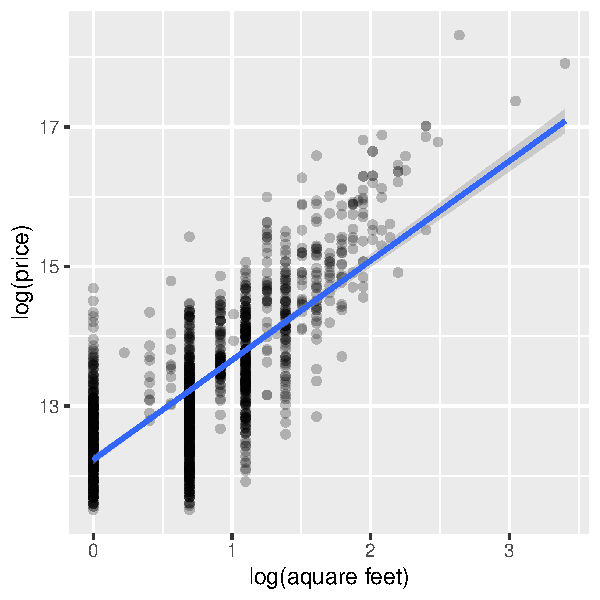
\includegraphics{about_files/figure-pdf/unnamed-chunk-5-1.pdf}
\end{center}

\begin{Shaded}
\begin{Highlighting}[]
\FunctionTok{tab\_model}\NormalTok{(slr\_LAprices2)}
\end{Highlighting}
\end{Shaded}

\begin{longtable}[]{@{}cccc@{}}
\toprule\noalign{}
\endhead
\bottomrule\noalign{}
\endlastfoot
~ & \multicolumn{3}{c@{}}{%
log(price)} \\
Predictors & Estimates & CI & p \\
(Intercept) & 12.23 & 12.18~--~12.29 & \textbf{\textless0.001} \\
bath {[}log{]} & 1.43 & 1.37~--~1.49 & \textbf{\textless0.001} \\
Observations & \multicolumn{3}{l@{}}{%
1594} \\
R\textsuperscript{2} / R\textsuperscript{2} adjusted &
\multicolumn{3}{l@{}}{%
0.577 / 0.577} \\
\end{longtable}

\end{tcolorbox}

\begin{tcolorbox}[enhanced jigsaw, toprule=.15mm, breakable, bottomtitle=1mm, coltitle=black, colback=white, arc=.35mm, left=2mm, leftrule=.75mm, opacitybacktitle=0.6, colframe=quarto-callout-warning-color-frame, colbacktitle=quarto-callout-warning-color!10!white, toptitle=1mm, titlerule=0mm, opacityback=0, title={Task 4}, rightrule=.15mm, bottomrule=.15mm]

Fit the multiple linear regression model using the \textbf{log transform
of all the variables} \texttt{price} (as the response) and both
\texttt{sqft} and \texttt{bath} (as the explanatory variables).
Calculate the point and interval estimates of the coefficients of the
two predictors separately. Compare their point and interval estimates to
those you calculated before. Can you account for the differences?

Click here to see the solution

\begin{Shaded}
\begin{Highlighting}[]
\NormalTok{mlr\_LAprices }\OtherTok{\textless{}{-}} \FunctionTok{lm}\NormalTok{(}\FunctionTok{log}\NormalTok{(price) }\SpecialCharTok{\textasciitilde{}} \FunctionTok{log}\NormalTok{(sqft) }\SpecialCharTok{+} \FunctionTok{log}\NormalTok{(bath), }\AttributeTok{data =}\NormalTok{ LAhomes)}
\FunctionTok{tab\_model}\NormalTok{(mlr\_LAprices,slr\_LAprices,slr\_LAprices2)}
\end{Highlighting}
\end{Shaded}

\begin{longtable}[]{@{}cccccccccc@{}}
\toprule\noalign{}
\endhead
\bottomrule\noalign{}
\endlastfoot
~ & \multicolumn{3}{c}{%
log(price)} & \multicolumn{3}{c}{%
log(price)} & \multicolumn{3}{c@{}}{%
log(price)} \\
Predictors & Estimates & CI & p & Estimates & CI & p & Estimates & CI &
p \\
(Intercept) & 2.51 & 2.00~--~3.03 & \textbf{\textless0.001} & 2.70 &
2.42~--~2.98 & \textbf{\textless0.001} & 12.23 & 12.18~--~12.29 &
\textbf{\textless0.001} \\
sqft {[}log{]} & 1.47 & 1.39~--~1.55 & \textbf{\textless0.001} & 1.44 &
1.40~--~1.48 & \textbf{\textless0.001} & & & \\
bath {[}log{]} & -0.04 & -0.13~--~0.05 & 0.389 & & & & 1.43 &
1.37~--~1.49 & \textbf{\textless0.001} \\
Observations & \multicolumn{3}{l}{%
1594} & \multicolumn{3}{l}{%
1594} & \multicolumn{3}{l@{}}{%
1594} \\
R\textsuperscript{2} / R\textsuperscript{2} adjusted &
\multicolumn{3}{l}{%
0.774 / 0.774} & \multicolumn{3}{l}{%
0.774 / 0.774} & \multicolumn{3}{l@{}}{%
0.577 / 0.577} \\
\end{longtable}

\end{tcolorbox}

\begin{tcolorbox}[enhanced jigsaw, toprule=.15mm, breakable, bottomtitle=1mm, coltitle=black, colback=white, arc=.35mm, left=2mm, leftrule=.75mm, opacitybacktitle=0.6, colframe=quarto-callout-warning-color-frame, colbacktitle=quarto-callout-warning-color!10!white, toptitle=1mm, titlerule=0mm, opacityback=0, title={Task 5}, rightrule=.15mm, bottomrule=.15mm]

Using the objective measures for model comparisons, which of the models
in task 2 ,3 and 4 would you favour? Is this consistent with your
conclusions in task 4?

Click here to see the solution

\begin{Shaded}
\begin{Highlighting}[]
\FunctionTok{tab\_model}\NormalTok{(mlr\_LAprices,slr\_LAprices,slr\_LAprices2,}\AttributeTok{show.aic =}\NormalTok{ T)}
\end{Highlighting}
\end{Shaded}

\begin{longtable}[]{@{}cccccccccc@{}}
\toprule\noalign{}
\endhead
\bottomrule\noalign{}
\endlastfoot
~ & \multicolumn{3}{c}{%
log(price)} & \multicolumn{3}{c}{%
log(price)} & \multicolumn{3}{c@{}}{%
log(price)} \\
Predictors & Estimates & CI & p & Estimates & CI & p & Estimates & CI &
p \\
(Intercept) & 2.51 & 2.00~--~3.03 & \textbf{\textless0.001} & 2.70 &
2.42~--~2.98 & \textbf{\textless0.001} & 12.23 & 12.18~--~12.29 &
\textbf{\textless0.001} \\
sqft {[}log{]} & 1.47 & 1.39~--~1.55 & \textbf{\textless0.001} & 1.44 &
1.40~--~1.48 & \textbf{\textless0.001} & & & \\
bath {[}log{]} & -0.04 & -0.13~--~0.05 & 0.389 & & & & 1.43 &
1.37~--~1.49 & \textbf{\textless0.001} \\
Observations & \multicolumn{3}{l}{%
1594} & \multicolumn{3}{l}{%
1594} & \multicolumn{3}{l@{}}{%
1594} \\
R\textsuperscript{2} / R\textsuperscript{2} adjusted &
\multicolumn{3}{l}{%
0.774 / 0.774} & \multicolumn{3}{l}{%
0.774 / 0.774} & \multicolumn{3}{l@{}}{%
0.577 / 0.577} \\
AIC & \multicolumn{3}{l}{%
44587.722} & \multicolumn{3}{l}{%
44586.467} & \multicolumn{3}{l@{}}{%
45584.113} \\
\end{longtable}

\end{tcolorbox}

\subsection{Part 2.}\label{part-2.}

You have been asked to determine the pricing of a New York City (NYC)
Italian restaurant's dinner menu such that it is competitively
positioned with other high-end Italian restaurants by analysing pricing
data that have been collected in order to produce a regression model to
predict the price of dinner.

Data from surveys of customers of 168 Italian restaurants in the target
area are available. The data can be found in the file
\texttt{restNYC.csv}.

Each row represents one customer survey from Italian restaurants in NYC
and includes the key variables:

\begin{itemize}
\tightlist
\item
  \texttt{Price} - price (in \$US) of dinner (including a tip and one
  drink)
\item
  \texttt{Food} - customer rating of the food (from 1 to 30)
\item
  \texttt{Decor} - customer rating of the decor (from 1 to 30)
\item
  \texttt{Service} - customer rating of the service (from 1 to 30)
\item
  \texttt{East} - dummy variable with the value 1 if the restaurant is
  east of Fifth Avenue, 0 otherwise
\end{itemize}

\begin{Shaded}
\begin{Highlighting}[]
\NormalTok{restNYC }\OtherTok{\textless{}{-}} \FunctionTok{read.csv}\NormalTok{(}\StringTok{"restNYC.csv"}\NormalTok{,}\AttributeTok{stringsAsFactors =}\NormalTok{ T)}
\end{Highlighting}
\end{Shaded}

\begin{tcolorbox}[enhanced jigsaw, toprule=.15mm, breakable, bottomtitle=1mm, coltitle=black, colback=white, arc=.35mm, left=2mm, leftrule=.75mm, opacitybacktitle=0.6, colframe=quarto-callout-warning-color-frame, colbacktitle=quarto-callout-warning-color!10!white, toptitle=1mm, titlerule=0mm, opacityback=0, title={Task 6}, rightrule=.15mm, bottomrule=.15mm]

Using the \texttt{ggpairs} function in the \texttt{GGally} package (see
the following code) we can generate an informative set of graphical and
numerical summaries which illuminate the relationships between pairs of
variables. Where do you see the strongest evidence of relationships
between \texttt{price} and the potential explanatory variables? Is there
evidence of multicollineatity in the data?

\begin{Shaded}
\begin{Highlighting}[]
\FunctionTok{library}\NormalTok{(GGally) }\CommentTok{\# Package to produce matrix of \textquotesingle{}pairs\textquotesingle{} plots and more!}
\NormalTok{restNYC}\SpecialCharTok{$}\NormalTok{East }\OtherTok{\textless{}{-}} \FunctionTok{as.factor}\NormalTok{(restNYC}\SpecialCharTok{$}\NormalTok{East) }\CommentTok{\# East needs to be a factor}
\CommentTok{\# Including the \textasciigrave{}East\textasciigrave{} factor}
\CommentTok{\# ggpairs(restNYC[, 4:8], aes(fill = East, alpha = 0.4),progress = F) }

\CommentTok{\# Without the \textasciigrave{}East\textasciigrave{} factor}
\FunctionTok{ggpairs}\NormalTok{(restNYC[, }\DecValTok{4}\SpecialCharTok{:}\DecValTok{7}\NormalTok{], }\FunctionTok{aes}\NormalTok{(}\AttributeTok{alpha =} \FloatTok{0.4}\NormalTok{),}\AttributeTok{progress =}\NormalTok{ F) }
\end{Highlighting}
\end{Shaded}

\begin{center}
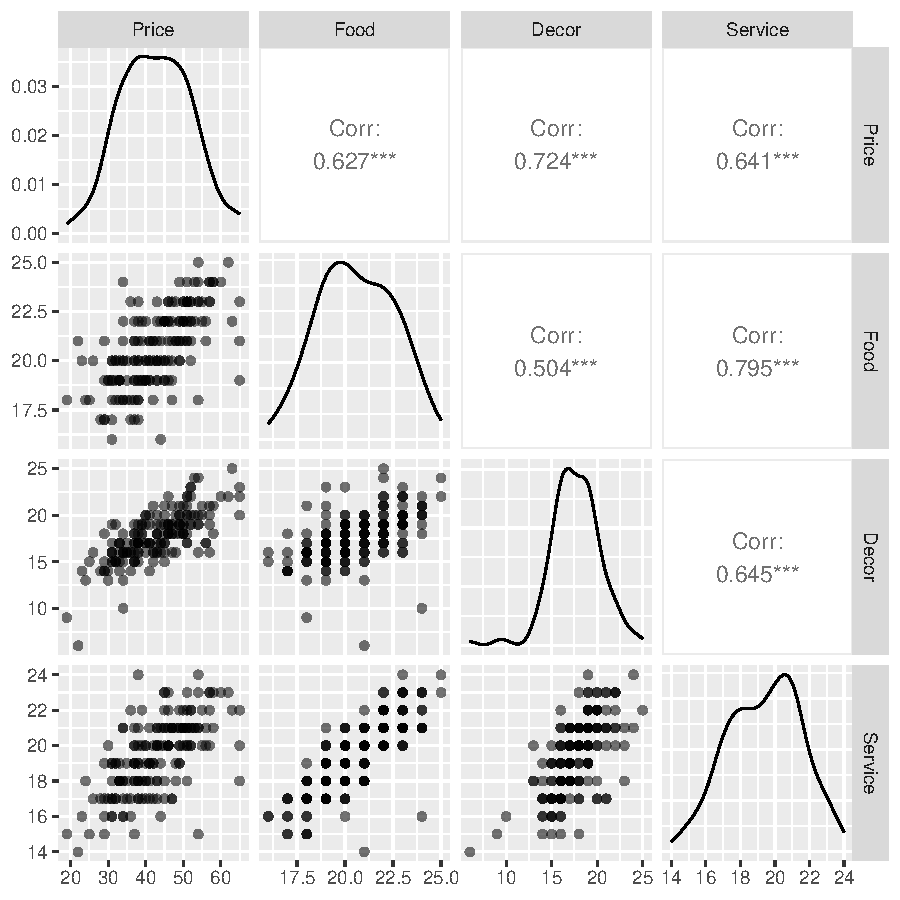
\includegraphics{about_files/figure-pdf/unnamed-chunk-9-1.pdf}
\end{center}

Solution

There seems to be a strong positive linear association between service
and food, which could lead to some collinearity issues.

\end{tcolorbox}

\begin{tcolorbox}[enhanced jigsaw, toprule=.15mm, breakable, bottomtitle=1mm, coltitle=black, colback=white, arc=.35mm, left=2mm, leftrule=.75mm, opacitybacktitle=0.6, colframe=quarto-callout-warning-color-frame, colbacktitle=quarto-callout-warning-color!10!white, toptitle=1mm, titlerule=0mm, opacityback=0, title={Task 7}, rightrule=.15mm, bottomrule=.15mm]

Fit the simple linear model with \texttt{Price} as the response and
\texttt{Service} as the predictor and display the fitted model on a
scatterplot of the data. Construct a confidence interval for the slope
parameter in the model.

Click here to see the solution

\begin{Shaded}
\begin{Highlighting}[]
\NormalTok{price\_serv\_LM }\OtherTok{\textless{}{-}} \FunctionTok{lm}\NormalTok{(Price  }\SpecialCharTok{\textasciitilde{}}\NormalTok{ Service  , }\AttributeTok{data =}\NormalTok{ restNYC)}
\FunctionTok{ggplot}\NormalTok{(restNYC, }\FunctionTok{aes}\NormalTok{(}\AttributeTok{x =}\NormalTok{ Service, }\AttributeTok{y =}\NormalTok{ Price)) }\SpecialCharTok{+}
  \FunctionTok{geom\_point}\NormalTok{() }\SpecialCharTok{+}
  \FunctionTok{geom\_jitter}\NormalTok{() }\SpecialCharTok{+}
  \FunctionTok{labs}\NormalTok{(}\AttributeTok{x =} \StringTok{"Service score"}\NormalTok{, }\AttributeTok{y =} \StringTok{"Price"}\NormalTok{)}\SpecialCharTok{+}
  \FunctionTok{geom\_smooth}\NormalTok{(}\AttributeTok{method =} \StringTok{"lm"}\NormalTok{)}
\end{Highlighting}
\end{Shaded}

\begin{center}
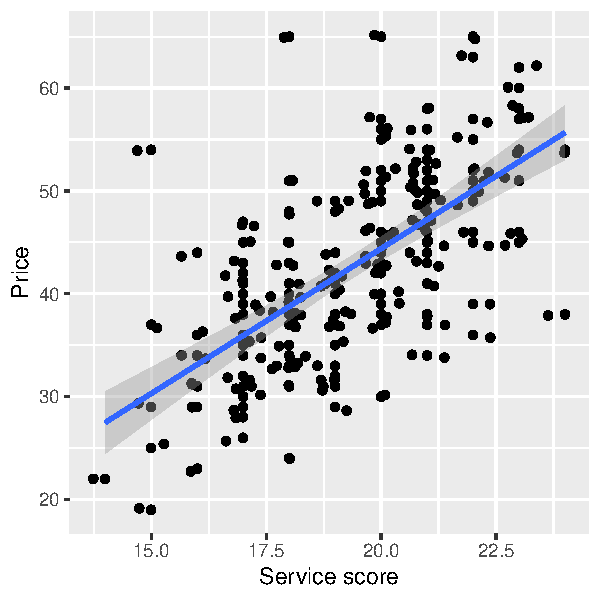
\includegraphics{about_files/figure-pdf/unnamed-chunk-10-1.pdf}
\end{center}

\begin{Shaded}
\begin{Highlighting}[]
\NormalTok{broom}\SpecialCharTok{::}\FunctionTok{tidy}\NormalTok{(price\_serv\_LM,}\AttributeTok{conf.int =}\NormalTok{ T)}
\end{Highlighting}
\end{Shaded}

\begin{verbatim}
# A tibble: 2 x 7
  term        estimate std.error statistic  p.value conf.low conf.high
  <chr>          <dbl>     <dbl>     <dbl>    <dbl>    <dbl>     <dbl>
1 (Intercept)   -12.0      5.11      -2.34 2.02e- 2   -22.1      -1.89
2 Service         2.82     0.262     10.8  7.88e-21     2.30      3.34
\end{verbatim}

\end{tcolorbox}

\begin{tcolorbox}[enhanced jigsaw, toprule=.15mm, breakable, bottomtitle=1mm, coltitle=black, colback=white, arc=.35mm, left=2mm, leftrule=.75mm, opacitybacktitle=0.6, colframe=quarto-callout-warning-color-frame, colbacktitle=quarto-callout-warning-color!10!white, toptitle=1mm, titlerule=0mm, opacityback=0, title={Task 8}, rightrule=.15mm, bottomrule=.15mm]

Now fit a multiple regressing model of \texttt{Price} on
\texttt{Service}, \texttt{Food}, and \texttt{Decor}. What happens to the
significance of \texttt{Service} when additional variables were added to
the model?

Click here to see the solution

\begin{Shaded}
\begin{Highlighting}[]
\NormalTok{price\_serv\_MLR }\OtherTok{\textless{}{-}} \FunctionTok{lm}\NormalTok{(Price  }\SpecialCharTok{\textasciitilde{}}\NormalTok{ Service }\SpecialCharTok{+}\NormalTok{ Food }\SpecialCharTok{+}\NormalTok{ Decor , }\AttributeTok{data =}\NormalTok{ restNYC)}
\FunctionTok{tab\_model}\NormalTok{(price\_serv\_MLR,}\AttributeTok{collapse.ci =}\NormalTok{ T)}
\end{Highlighting}
\end{Shaded}

\begin{longtable}[]{@{}
  >{\centering\arraybackslash}p{(\columnwidth - 4\tabcolsep) * \real{0.3333}}
  >{\centering\arraybackslash}p{(\columnwidth - 4\tabcolsep) * \real{0.3333}}
  >{\centering\arraybackslash}p{(\columnwidth - 4\tabcolsep) * \real{0.3333}}@{}}
\toprule\noalign{}
\endhead
\bottomrule\noalign{}
\endlastfoot
~ &
\multicolumn{2}{>{\centering\arraybackslash}p{(\columnwidth - 4\tabcolsep) * \real{0.6667} + 2\tabcolsep}@{}}{%
Price} \\
Predictors & Estimates & p \\
(Intercept) & \begin{minipage}[t]{\linewidth}\raggedright
-24.64\\
(-34.03~--~-15.25)\strut
\end{minipage} & \textbf{\textless0.001} \\
Service & \begin{minipage}[t]{\linewidth}\raggedright
0.14\\
(-0.65~--~0.92)\strut
\end{minipage} & 0.733 \\
Food & \begin{minipage}[t]{\linewidth}\raggedright
1.56\\
(0.82~--~2.29)\strut
\end{minipage} & \textbf{\textless0.001} \\
Decor & \begin{minipage}[t]{\linewidth}\raggedright
1.85\\
(1.42~--~2.28)\strut
\end{minipage} & \textbf{\textless0.001} \\
Observations &
\multicolumn{2}{>{\raggedright\arraybackslash}p{(\columnwidth - 4\tabcolsep) * \real{0.6667} + 2\tabcolsep}@{}}{%
168} \\
R\textsuperscript{2} / R\textsuperscript{2} adjusted &
\multicolumn{2}{>{\raggedright\arraybackslash}p{(\columnwidth - 4\tabcolsep) * \real{0.6667} + 2\tabcolsep}@{}}{%
0.617 / 0.610} \\
\end{longtable}

\end{tcolorbox}

\begin{tcolorbox}[enhanced jigsaw, toprule=.15mm, breakable, bottomtitle=1mm, coltitle=black, colback=white, arc=.35mm, left=2mm, leftrule=.75mm, opacitybacktitle=0.6, colframe=quarto-callout-warning-color-frame, colbacktitle=quarto-callout-warning-color!10!white, toptitle=1mm, titlerule=0mm, opacityback=0, title={Task 9}, rightrule=.15mm, bottomrule=.15mm]

What is the correct interpretation of the coefficient on
\texttt{Service} in the linear model which regresses \texttt{Price} on
\texttt{Service}, \texttt{Food}, and \texttt{Decor}?

See solution

After controlling for \texttt{Food} and \texttt{Decor}, a 1-point
increase in the \texttt{Service} rating is associated with an estimated
\$0.135 increase in the. average Price, but this effect is not
statistically significant (p \(>\) 0.05)

\end{tcolorbox}



\end{document}
